\chapter{Simulation Modeling}
In this chapter we will answer four fundamental questions, which are:
\begin{compactitemize}
    \item What is \textbf{Simulation}?
    \item What is a \textbf{System}?
    \item What is a \textbf{Model}?
    \item What is a \textbf{Discrete-Event} Simulation?
\end{compactitemize}

\section{What is Simulation?}

\textbf{Simulation} can be defined, in a very general sense, as the process of designing a model of a real system and conducting experiments on that model with the goal of:
\begin{compactitemize}
    \item understanding the behaviour of the system over time;
    \item evaluating different strategies for the operation of the system.
\end{compactitemize}

\begin{wrapfigure}{r}{0.5\textwidth}
    \centering
    \vspace{-10pt}
    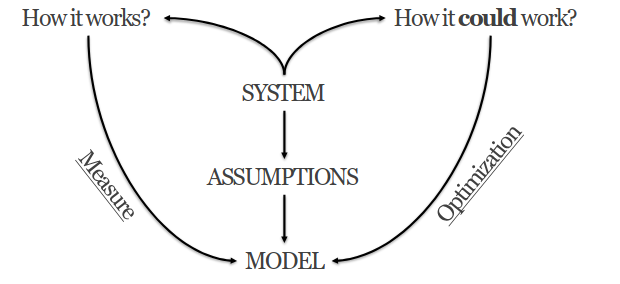
\includegraphics[width=\linewidth]{images/L2.png}
    \label{fig:Scaled Dot Product Attention}
    \vspace{-10pt}
\end{wrapfigure}
This is a deliberately broad, high-level definition: the central idea is that, instead of intervening directly on the real system, a simplified representation of it is built and the effects of decisions are studied in a controlled environment.

More formally, a simulation is the imitation of the operation of a real system along the time axis. It first of all requires the definition of a set of assumptions about the system, then the generation of an \emph{artificial history} of the system itself and finally the observation of that history to draw inferences about the operating characteristics of the system.

\subsection{Objectives of Simulation}

The use of simulation essentially responds to two main objectives.
The first is observing the behaviour of a system as it is, that is, a classic \textbf{AS-IS} analysis. In this case we want to measure performance metrics, identify bottlenecks or understand the internal dynamics of the system.

The second objective is the optimization of the system, in a \textbf{TO-BE} logic. Here simulation is used to answer \emph{what-if} questions: what would happen if we modified a component of the system? If we changed a decision rule? If we introduced a new technology? In this way it is possible to evaluate alternatives without having to implement them in the real world.

\subsection{Simulation as a Process: System, Model, Simulation}

It is fundamental to clarify that simulation is a \textbf{process}, not a single object.
The process follows a very precise conceptual scheme:

\begin{center}
\textbf{System} $\longrightarrow$ \textbf{Model} $\longrightarrow$ \textbf{Simulation}
\end{center}

The \textbf{system} is the real system we want to study, for example a bank, a warehouse or a supply chain.
From the system a \textbf{model} is built, which is nothing but an \emph{approximation} and a \emph{simplification} of the real system. The model does not include everything, but only those aspects that are relevant to the objectives of the study.
Finally, from the model we obtain the \textbf{simulation}, that is, the execution of the model over time to produce artificial data to be analysed.

This point is crucial: \emph{the simulation does not learn anything directly from the real system}, but only from what the model represents. Consequently, the quality of the simulation results depends entirely on the quality of the model.

\subsection{Simulation Techniques}

In some cases the models are simple enough to be analysed with classic mathematical tools, such as probability, differential calculus or mathematical programming. In these situations it is possible to obtain exact analytical solutions.

However, many real systems show a high level of complexity: non-linear behaviours, multiple interactions, random events and temporal dependencies make an analytical solution impossible or impractical. In these cases we resort to simulation models based on computation.

\subsection{When Simulation Is Appropriate}

Simulation is a particularly suitable tool when we want to study the internal operation of a complex system, analyse the effect of organizational or environmental changes, understand how variations of the inputs affect the outputs, verify analytical solutions or support education and training activities.

In all these cases, the main advantage is the possibility of experimenting without risks for the real system.
\begin{figure}[H]
    \centering
    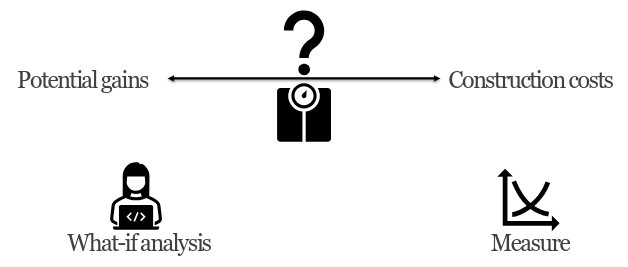
\includegraphics[width=0.6\textwidth]{images/L1.png}
    \label{fig:student_markov_chain}
\end{figure}
\subsection{When Simulation Is \emph{Not} the Appropriate Tool}

It is equally important to understand when \textbf{simulation is not the right tool}. An improper use of simulation can lead to misleading results, waste of resources and wrong decisions.

First of all, simulation is not appropriate when the problem can be easily solved with common sense or with a simple analytical solution. In these cases, building a simulation model would be unnecessarily expensive.

Simulation is not suitable either when carrying out direct experiments on the real system is cheaper, faster or more informative than building a model.

Another important limitation concerns the availability of resources: if there is not enough time, data or expertise, the result will be a poor and unreliable model.

The most critical point, however, is the following: \textbf{if the model is not validated, the simulation is not reliable}.
Simulation works exclusively on the model. If the model does not adequately represent the real system, then the simulation will inevitably produce wrong results. In this case, it does not matter how sophisticated the simulation is or how accurate the analysis is: the conclusions will be wrong because they are based on a wrong representation of the system.

In other words:
\begin{center}
\emph{Invalid model $\Rightarrow$ invalid simulation $\Rightarrow$ invalid decisions}
\end{center}

For this reason, model validation is one of the most delicate and fundamental steps in every simulation study.

Finally, simulation is not appropriate when the level of detail required to answer the questions of interest is so high that it makes the model excessively complex, expensive and difficult to interpret.

\subsection{Advantages and Disadvantages of Simulation}

Among the main advantages of simulation is the possibility of exploring new operating policies without disturbing the real system, testing new designs without committing resources, verifying hypotheses about the behaviour of the system and better understanding the interactions between variables and the bottlenecks.

On the other hand, simulation requires specific expertise, can be expensive in terms of time and computational resources, and produces results that are always estimates or approximations, affected by the variability of the inputs.

\subsection{Areas of Application}

Simulation finds application in numerous contexts, including traffic management, the introduction of new automation technologies, the management of disruptions in demand, supply chain design, last-mile logistics, financial evaluations and optimal control problems.

In all these cases, simulation provides a safe environment in which to experiment and make informed decisions, provided that the model on which it is based is accurately built and validated.

\section{What is a System?}

In order to build a simulation model it is fundamental to first clarify what is meant by \textbf{system}. In general, a system is defined as a set of entities that interact with each other in a regular or interdependent way with the purpose of achieving a certain goal.

This definition highlights three essential elements: the existence of several components, the interaction between these components and the presence of a goal or a function that the system must perform. A system, therefore, is not simply a collection of objects, but an organized structure in which the parts mutually influence the overall behaviour.

A classic example is an industrial production system, such as a car assembly line. In this case, the system is the entire production process; the entities are machines, workers and components; the goal is the production of high-quality vehicles at a certain rate.

\subsection{System, State, and Environment}

The practical meaning of system always depends on the objectives of the simulation study. Depending on what we want to analyse, the way in which the system is delimited changes.

The \textbf{state} of a system is defined as the set of variables needed to describe it at a given instant of time. If the state is known, then the future behaviour of the system can be determined (in a probabilistic or deterministic sense) from it.

The \textbf{environment} includes everything that is external to the system but that can influence its behaviour. The distinction between system and environment is not absolute, but depends on the choices of the modeller and on the purpose of the simulation.

The \textbf{boundary} represents the conceptual border that separates the system from the environment. For example, in a simulation of a bank, the customer arrival process can be considered part of the environment, since it is not under the control of the bank, while the service policy (number of counters, priority rules) is part of the system.

\subsection{Components of a System}

To understand and model a system it is necessary to identify its fundamental components. A first component is the \textbf{entity}, that is, an object of interest within the system, such as a customer, a product or a vehicle.

Each entity is characterized by one or more \textbf{attributes}, which describe its properties. In the case of a banking system, for example, the attributes of a customer can include the account balance, the credit rating or a unique identifier.

An \textbf{activity} represents a period of time during which a specific operation takes place, such as the delivery of a service, a payment or a processing phase. Activities have a duration that can be deterministic or random.

An \textbf{event}, instead, is an instantaneous occurrence that causes a change in the state of the system. The arrival of a customer or the completion of a service are typical examples of events. Events can be exogenous, if they originate from the environment, or endogenous, if they are generated by the system itself.

Finally, the \textbf{state variables} are the minimal set of variables capable of completely describing the state of the system at every instant of time, such as the number of busy servers or the length of a queue.

It is important to underline that there is no universal list of components valid for every system: the choice always depends on the objectives of the simulation study.
\begin{figure}[H]
    \centering
    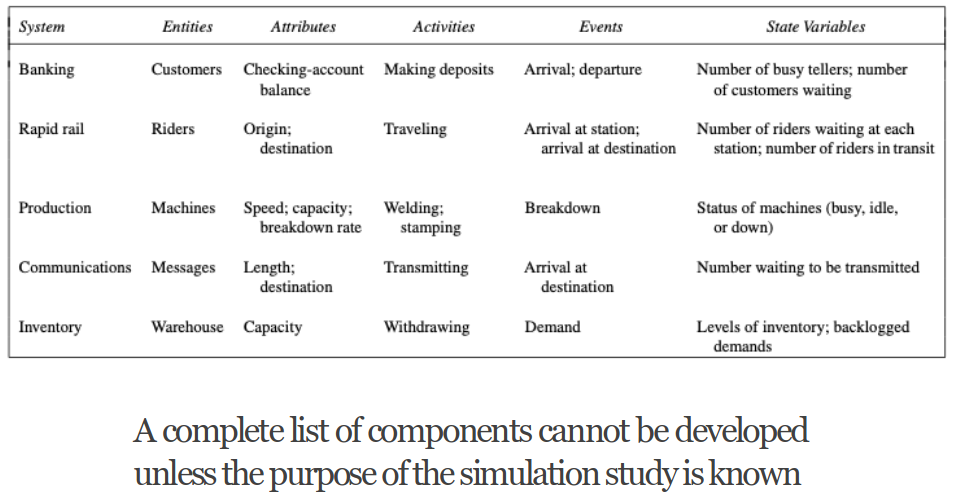
\includegraphics[width=0.8\textwidth]{images/L3.png}
    \label{fig:student_markov_chain}
\end{figure}
\subsection{Discrete and Continuous Systems}

A system is called \textbf{discrete} if its state variables change only at discrete instants of time, typically when events occur. Classic examples are a bank, a warehouse or a production line.

A system is instead \textbf{continuous} if the state variables evolve continuously over time, as in the case of the water level in a dam or the trend of a financial variable.

This distinction is conceptual and does not impose a rigid correspondence between system and model. A continuous system can be approximated through a discrete model and vice versa. The choice depends on the nature of the system and on the purpose of the analysis.

In conclusion, understanding what is meant by system, how to define its boundaries and which components to include is an essential step before building a model and, subsequently, a reliable simulation. A wrong definition of the system inevitably leads to inadequate models and to simulations that are not representative of reality.

\section{What is a Model?}

After having defined what a \textbf{system} is, the next step in the simulation process is the construction of a \textbf{model}. A model is a representation of a system, built with the purpose of studying its behaviour, understanding its internal dynamics or predicting its performance under different decision policies.

By definition, a model is a \textbf{simplification} of the real system. It is neither possible nor desirable to include every detail of the real world: the goal is instead to keep only the elements relevant to the problem being analysed. However, this simplification must be carefully balanced, since the model must be detailed enough to allow valid and reliable conclusions.

In this sense the famous principle of George Box applies: \emph{“All models are wrong, but some are useful”}. Every model is inevitably “wrong” because it does not reproduce reality perfectly, but it can still be extremely useful if it captures the essential aspects of the system that influence the behaviour of interest.

\subsection{Purpose of a Model}

A model is built for a very specific purpose. In some cases the goal is to understand the relations between the components of the system; in other cases we want to predict the performance of the system under new operating conditions or new decision policies.

Although in principle a system could be studied through direct experiments, in practice this approach is often impractical. The system might not exist yet, as in the case of a new production plant, or it might be too expensive, risky or complex to experiment on directly. In these cases, the model becomes the main analysis tool.

It is important to underline that, if the purpose of the study changes, the model must change too. A model built to analyse the waiting times of a system might not be suitable for evaluating energy costs or robustness to failures.

\subsection{Model Complexity and Trade-offs}

Building a model requires a compromise between simplicity and realism. A model that is too simple risks neglecting important variables, leading to misleading conclusions. On the contrary, an excessively complex model can become difficult to understand, implement and validate, paradoxically ending up being as opaque as the real system.

As the level of detail increases, so do the requirements in terms of data, development time and computational costs. For this reason, a good model is not the most complex one possible, but the one that includes only what is necessary to answer the questions posed by the study.

\subsection{Classification of Models}

Models can be classified along several dimensions, depending on their fundamental characteristics.

A first distinction is between \textbf{physical models} and \textbf{mathematical models}. Physical models are tangible, scaled representations of the real system. Mathematical models instead describe the system through logical and quantitative relations, using equations and mathematical symbols. In the context of simulation, we work almost exclusively with mathematical models.

Models can also be \textbf{static} or \textbf{dynamic}. A static model represents the system at a single instant or without a real temporal evolution, as in the case of some Monte Carlo simulations. A dynamic model, instead, explicitly represents the change of the state of the system over time and is the most common type of model in the simulation of real processes.

A further distinction concerns \textbf{deterministic} and \textbf{stochastic} models. In deterministic models there are no random variables and, for the same input, the output is always identical. In stochastic models, instead, some components are random and the outputs are therefore estimates of the true performance of the system.

Finally, models can be \textbf{discrete} or \textbf{continuous}. In discrete models the state of the system changes only at discrete instants of time, while in continuous models the state evolves continuously. There is no rigid correspondence between system and model: a continuous system can be modelled in a discrete way and vice versa, depending on the objectives of the study.

\subsection{Models and Simulation}

In the simulation process, the model occupies a central position. We start from a real system, which is approximated through a model; the model is then used to generate a simulation, that is, an “artificial history” of the system. The conclusions drawn from the simulation depend entirely on the quality of the model.

If the model is not appropriate or not validated, the simulation will produce misleading results. In other words, a simulation can never compensate for a bad model: precise results obtained from a wrong model lead to wrong decisions. For this reason, the construction and validation of the model are among the most critical phases of any simulation study.
\begin{figure}[H]
    \centering
    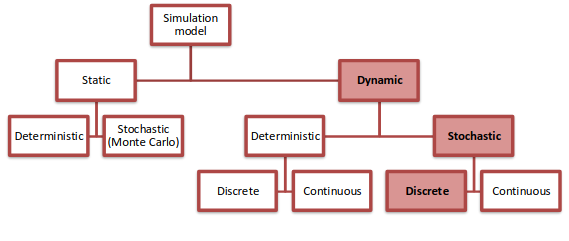
\includegraphics[width=0.8\textwidth]{images/L4.png}
    \label{fig:student_markov_chain}
\end{figure}

\section{What is a Discrete-Event Simulation (D.E.S.)}

A Discrete-Event Simulation (DES) is a specific class of simulation models used to represent systems that evolve over time through the occurrence of discrete events. In this framework, the state of the system does not change continuously, but only at distinct points in time, when specific events occur.

Formally, a discrete-event simulation models a system whose state variables change instantaneously at separate points in time. These points in time are called \emph{events}. Each event corresponds to a meaningful occurrence in the system, such as the arrival of an entity, the start of a service, or the completion of an activity. When an event occurs, the state of the system may change as a consequence.

Unlike analytical models, DES does not aim to solve equations analytically. Instead, it relies on numerical methods and computational procedures. Models are not \emph{solved}, but rather \emph{run}. By executing the simulation model, an artificial history of the system is generated, and observations are collected over simulated time. These observations are then analysed to obtain estimates of the true performance measures of the real system.

\subsection{Example: Single-Server Queue}

To illustrate the concept of discrete-event simulation, consider a simple service system with a single server, such as a one-person barbershop, a bank teller, or an information desk. The objective of the study is to estimate the expected average delay experienced by customers waiting in line. The delay is defined as the time interval between the arrival of a customer and the start of service.

The system is described through a set of state variables, such as the status of the server (idle or busy), the queue length, and the arrival times of customers. The evolution of the system is driven by events. In this example, three types of events are sufficient to fully capture the system dynamics: the \textbf{arrival} of a customer, the \textbf{start of service}, and the \textbf{departure} of a customer, which coincides with the completion of service. Each of these events may modify the system state when it occurs.

This example highlights the key characteristics of DES: state changes occur only at event times, and the system dynamics are fully determined by the sequence and timing of events.
\begin{figure}[H]
    \centering
    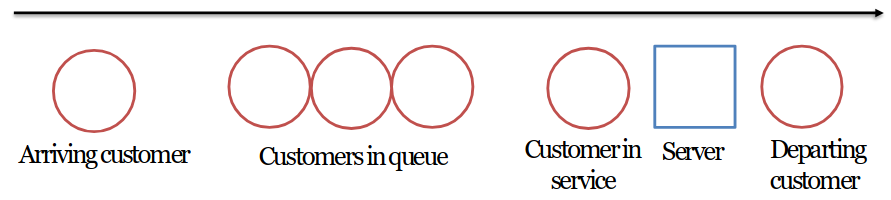
\includegraphics[width=0.8\textwidth]{images/L5.png}
    \label{fig:student_markov_chain}
\end{figure}
\subsection{Steps in a Simulation Study}

A discrete-event simulation study follows a structured process, which can be divided into four main phases: 
\begin{compactitemize}
    \item \textbf{Discovery}
    \item \textbf{Model Building}
    \item \textbf{Run}
    \item \textbf{Implementation}
\end{compactitemize}
The first phase is the discovery and orientation phase. This phase begins with problem formulation. The problem must be clearly understood before any modelling effort starts. A common mistake at this stage is developing a solution without a well-defined problem. Along with problem formulation, the objectives of the study are defined and an overall project plan is established. The objectives specify which questions the simulation is expected to answer, while the project plan addresses practical aspects such as time constraints, costs, and required resources.

The second phase is the model building phase, which is the core of the simulation study. It starts with model conceptualization, where the essential features of the system are identified and translated into a conceptual model. This involves selecting the basic assumptions that characterise the system and deciding which elements are relevant for the study. Model construction is as much an art as it is a science: a common practice is to start with a simple model and progressively introduce complexity, ensuring that each added detail contributes useful information.

\begin{wrapfigure}{r}{0.6\textwidth}
    \centering
    \vspace{-10pt}
    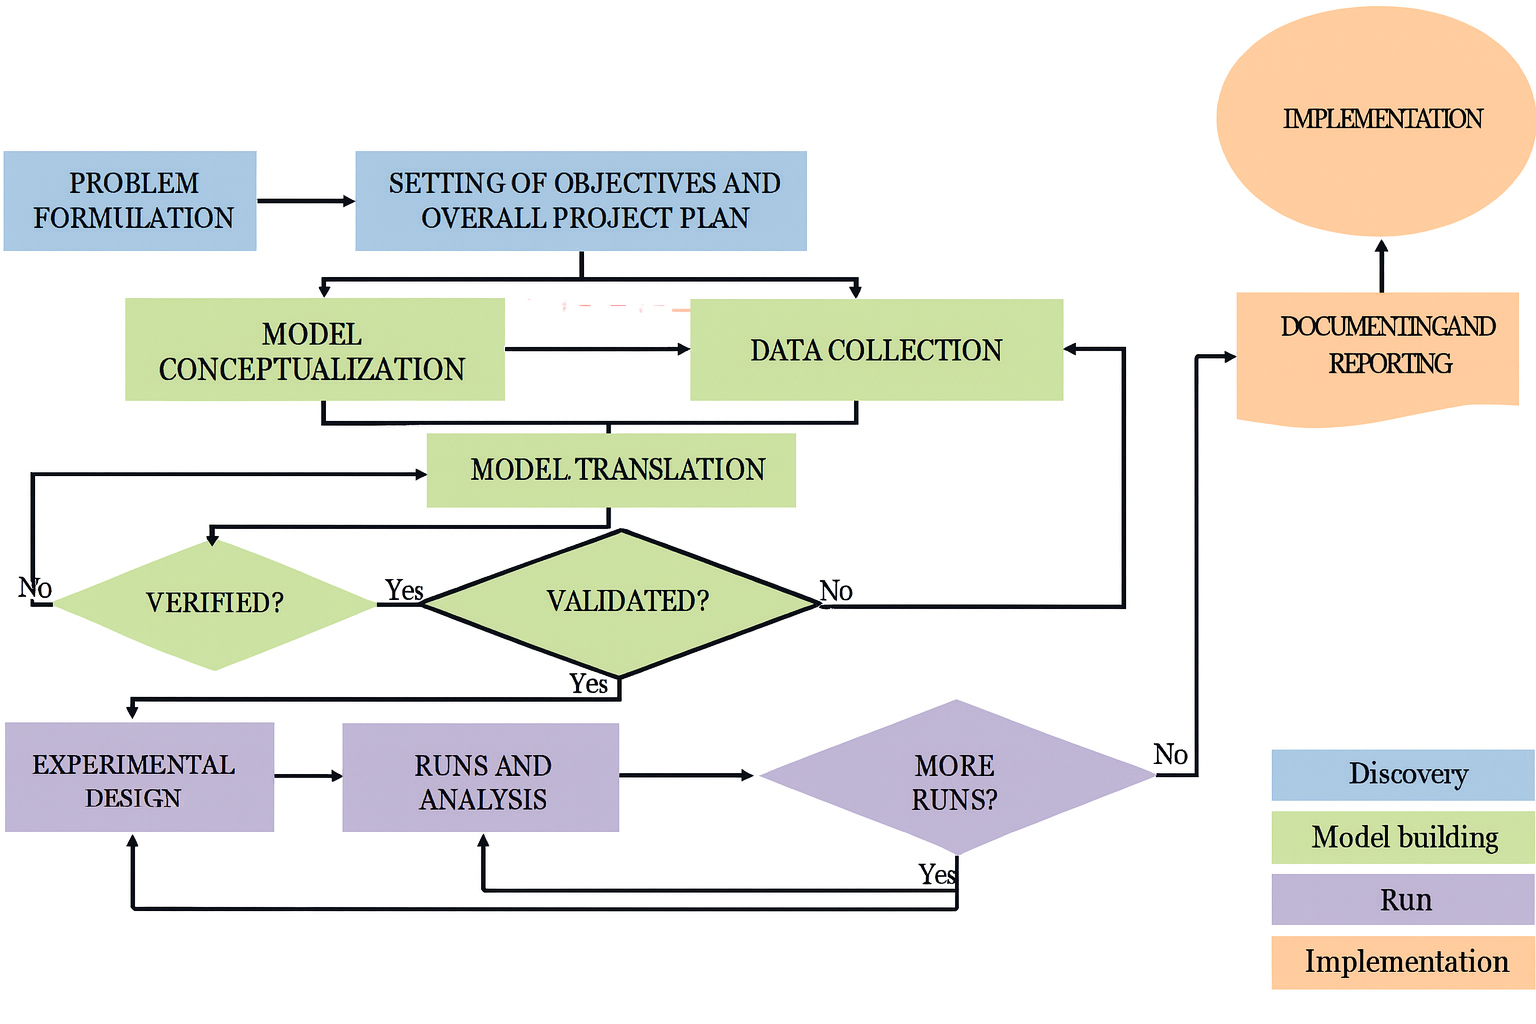
\includegraphics[width=\linewidth]{images/L6.png}
    \label{fig:Scaled Dot Product Attention}
    \vspace{-10pt}
\end{wrapfigure}
Data collection is tightly coupled with model building. As the model evolves, different types and levels of input data may be required. Because data collection can be time-consuming and expensive, it should start early and proceed in parallel with model development. Once the conceptual model and data are available, the model is translated into a software implementation. In this course, this translation is performed using Python and the SimPy library.

A crucial part of the model building phase is verification and validation. Model verification answers the question: “Is the model implemented correctly?” It focuses on whether the code faithfully represents the conceptual model and behaves as intended. Model validation, instead, addresses a deeper question: “Does the model accurately represent the real system?” Validation is achieved through calibration and comparison between simulated outputs and observed system behaviour. Discrepancies are not necessarily failures; they often provide valuable insight into the system and guide improvements to the model. This is the most critical step of the entire simulation process: an invalid model inevitably leads to invalid decisions, regardless of how well the simulation is executed.

The third phase is the run phase. At this stage, the validated model is used to perform experiments. An experimental design is defined, specifying the decision alternatives to be evaluated. For each alternative, key choices must be made, such as the length of the simulation run, the presence and duration of a warm-up period, and the number of independent replications. The objective is to obtain unbiased performance estimates with sufficiently low variance.

The final phase is the implementation phase. This includes documentation and reporting, which ensure that the model and results are understandable, reproducible, and reusable in the future. Clear documentation also supports future modifications and extensions of the model. Implementation refers to the actual adoption of a selected alternative in the real system. The success of this phase depends entirely on the quality of all previous steps: a well-defined problem, a valid model, and a rigorous experimental analysis.

In summary, a discrete-event simulation is a powerful and flexible tool for analysing complex dynamic systems. However, its effectiveness relies on a disciplined modelling process, careful validation, and a clear understanding of the limits and assumptions underlying the model.
